\begin{definition}(Group) \leavevmode \\
    A group is an ordered pair $(G, *)$ where $G$ is a set and $*$ is a mapping from $G\times G$ to $G$ (called a binary operation) satisfying the following:
    \begin{enumerate}
        \item $\forall a, b, c \in G ~~a*(b*c)=(A*b)*c$ (associativity)
        \item $\exists e \in G \st e*a=a=a*e ~~\forall a \in G$ (identity element)
        \item $\forall a \in G, \exists a^{-1} \in G \st a*a^{-1}=e=a^{-1}*a$ (inverse element)
    \end{enumerate}
\end{definition}

From now on we write $a*b = ab$.

\begin{definition}[Permutations] \leavevmode \\
    Let $\Omega$ be a nonempty set. The mapping $\sigma: \Omega \to \Omega$ is a permutation of $\Omega$ if $\sigma$ is a bijection.
\end{definition} %
\begin{wrapfigure}{l}{0.35\textwidth} % l = left, r = right
  \centering
  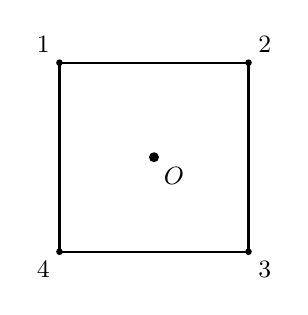
\begin{tikzpicture}[scale=1.2, every node/.style={font=\small}]
    % square centered at origin
    \coordinate (A) at (-1,-1); % 1
    \coordinate (B) at ( 1,-1); % 2
    \coordinate (C) at ( 1, 1); % 3
    \coordinate (D) at (-1, 1); % 4
    \draw[thick] (A) -- (B) -- (C) -- (D) -- cycle;

    % vertex dots + labels
    \fill (A) circle (1pt); \node[below left]  at (A) {4};
    \fill (B) circle (1pt); \node[below right] at (B) {3};
    \fill (C) circle (1pt); \node[above right] at (C) {2};
    \fill (D) circle (1pt); \node[above left]  at (D) {1};

    % origin
    \fill (0,0) circle (1.5pt);
    \node[below right] at (0,0) {$O$};
  \end{tikzpicture}
\end{wrapfigure}

Here is a square centered at the origin. Take a copy of the square, move it around in 3-space, and lay it back down to cover the original square. This is called a rigid motion of the square, or a symmetry of the square. This creates a permutation of the vertices. How many symmetries are possible?

%%%%%%%%%%%%%%%%figures go here %%%%%%%%%%%%%%%%

For the arbitrary symmetry of the square, we have 4 choices where to find 1. Once we know where vertex 1 is (say, vertex i), then vertex 2 can be one of 2 places. This gives $4\times2$ symmetries. Consider the regular $n$-gon centered at the origin. How many symmetries do we have? $2n$.

\begin{fact} [Properties of Permutations] \leavevmode \\
\begin{enumerate}
    \item Functional composition is associative. For mappings $\sigma, \tau, \mu$
    $$\sigma \circ (\tau \circ \mu) = (\sigma \circ \tau) \circ \mu$$
    \item The identity mapping on any set ($I(x) = x$) is a bijection of that set.
    \item If $\sigma$ is a bijection from a set $\Omega$ to $\Omega$, then there is a bijection of $\Omega$ called $\sigma^{-1}$ such that $\sigma \circ \sigma^{-1} = I = \sigma^{-1} \circ \sigma$.
\end{enumerate}
\end{fact}

\begin{definition}[Order] \leavevmode \\
    For $a\in G$, where $G$ is a group, the order of $a$, denoted $|a|$, is the smallest positive integer $k$ such that $a^k = e$ if such a $k$ exists. If no such $k$ exists, then we say $a$ has infinite order and $|a| = \infty$.
\end{definition}

\begin{notation}[Cycle Decomposition] \leavevmode \\
    A permutation $\sigma$ of a set $\Omega$ can be written as a product of disjoint cycles. For example, if $\sigma$ is a permutation of $\{1,2,3,4,5\}$ such that $\sigma(1)=3$, $\sigma(3)=1$, $\sigma(2)=5$, $\sigma(5)=2$, and $\sigma(4)=4$, then we can write $\sigma = (1~3)(2~5)(4)$. The order of a cycle is the number of elements in the cycle. The order of a permutation is the least common multiple of the orders of the disjoint cycles.
\end{notation}

\begin{example} \leavevmode \\
  If $\sigma = (1~2)(3~2),$ then $\sigma(3) = 1$. \\
  If $\mu = (3~2)(1~2),$ then $\mu(3) = 2$. \\
  $S_n$ is not abelian for $n \geq 3$.
\end{example}
